\documentclass[10pt,a4paper]{article}
% Gestaltung: gemeinsamer Akademie-Stil (Schriften, Farben, Kopf-/Fusszeile, Kaesten, Tabellen)
\usepackage{../stil/akademie}
\special{dvipdfmx:config z 0}   % ohne Kompression, maximale Druckkompatibilitaet
\usepackage{hyperref}\hypersetup{hidelinks,pdftitle={Pending Orders – Standard Tier},pdfsubject={Buy Limit, Sell Limit, Buy Stop, Sell Stop}}
\akdokument{Pending Orders}\akreihe{Trading-Grundlagen}

% ---- Raster der Ordertyp-Seiten -----------------------------------------
% Links eine Randspalte fuer die Zwischenueberschriften (\labw, akademie.sty),
% rechts der Text. Chart, Absaetze und Beispiel beginnen alle an derselben Kante.
\def\cu{0.6mm}% Massstab der grossen Charts: 1 Einheit = 1 px des Plattformbilds
% charts.tikz -- Vektor-Nachbau der vier Plattform-Chartbilder
% (img-pending-order-{bl,sl,bs,ss}.png, 174 x 96 px; Ursprung unten links,
% 1 Einheit = 1 px).  Je Bild 37 Rechtecke (Balken und Stiele), 2 Kreise
% (Kugeln: links rot = Kurs jetzt, rechts gruen = At price), 1 Dreieck
% (Richtung danach).  Farben: pfgruen, pfrot, pfgrau (abgedunkelte graue
% Kerzen fuer weissen Grund), definiert in der .tex.
%
% AUTOMATISCH ERZEUGT von tools/charts_aus_pdf.py aus
% originals/Pending-Orders-Guide_ORIGINAL.pdf (Seiten 1, 3, 4, 5).
% Alle Werte sind bitgenau aus dem Inhaltsstrom zurueckgerechnet.

\newcommand{\chartbl}{%
  \fill[pfrot] (14,66) rectangle (16.367,89.525);
  \fill[pfrot] (52.702,83.5) circle (3.651);
  \fill[pfrot] (51.497,44) rectangle (53.874,83.5);
  \fill[pfrot] (19,62) rectangle (21,85.624);
  \fill[pfrot] (23,58.683) rectangle (25.376,82);
  \fill[pfrot] (31,54.599) rectangle (33.502,78);
  \fill[pfrot] (39.251,49) rectangle (41.624,72.37);
  \fill[pfrot] (27,46.475) rectangle (29.367,70);
  \fill[pfrot] (35.125,46.375) rectangle (37.623,70);
  \fill[pfrot] (43.252,43.124) rectangle (45.75,66.75);
  \fill[pfrot] (47.371,38.251) rectangle (49.873,61.873);
  \fill[pfgrau] (64,39) rectangle (66,58.624);
  \fill[pfgrau] (55.498,38.251) rectangle (58,57.748);
  \fill[pfgrau] (68,36) rectangle (70,55.376);
  \fill[pfgrau] (76,36) rectangle (78.376,55.317);
  \fill[pfgrau] (59.655,33.37) rectangle (62,52.736);
  \fill[pfgrau] (88.251,32.63) rectangle (90.624,52);
  \fill[pfgrau] (80,31.699) rectangle (82.502,51);
  \fill[pfgrau] (72,30) rectangle (74.365,49.525);
  \fill[pfgrau] (96.37,29.251) rectangle (98.872,48.873);
  \fill[pfgrau] (104.498,31) rectangle (107,48.873);
  \fill[pfgrau] (84.125,28.375) rectangle (86.623,48);
  \fill[pfgrau] (92.251,27.849) rectangle (94.749,47);
  \fill[pfgrau] (100.498,23.604) rectangle (102.875,43);
  \fill[pfgruen] (152.349,83) -- (164.69,83) -- (158.476,89) -- cycle;
  \fill[pfgruen] (151.125,51.251) rectangle (153.623,70.876);
  \fill[pfgruen] (155.251,49) rectangle (157.624,68.159);
  \fill[pfgruen] (163.373,48) rectangle (165.875,69);
  \fill[pfgruen] (159.251,45) rectangle (161.749,64.151);
  \fill[pfgruen] (147,44) rectangle (149.502,63.401);
  \fill[pfgruen] (139,37.475) rectangle (141.365,57);
  \fill[pfgruen] (143,35) rectangle (145.376,54.422);
  \fill[pfgruen] (134,31.683) rectangle (136.376,51);
  \fill[pfgruen] (129.125,27) rectangle (131.502,46.158);
  \fill[pfgruen] (121,23.578) rectangle (123.376,43);
  \fill[pfgruen] (109.881,7.5) circle (3.594);
  \fill[pfgruen] (108.62,7.5) rectangle (111,38.962);
  \fill[pfgruen] (125,20.37) rectangle (127.345,39.736);
  \fill[pfgruen] (117,18) rectangle (119,37.376);
  \fill[pfgruen] (113,14.498) rectangle (115,34);
}
\newcommand{\chartsl}{%
  \fill[pfrot] (54,44) rectangle (56.376,63.422);
  \fill[pfrot] (67.493,15.5) circle (3.457);
  \fill[pfrot] (66.125,15.5) rectangle (68.625,60.962);
  \fill[pfrot] (58,41.599) rectangle (60.502,61);
  \fill[pfrot] (62.125,37.5) rectangle (64.502,57);
  \fill[pfrot] (50,36.624) rectangle (52,56);
  \fill[pfrot] (41.635,30) rectangle (44,49.525);
  \fill[pfrot] (46,27.624) rectangle (48,47);
  \fill[pfrot] (37,24.251) rectangle (39,43.875);
  \fill[pfrot] (32,19.376) rectangle (34,39);
  \fill[pfrot] (24,16.125) rectangle (26,35.749);
  \fill[pfrot] (11.373,13) rectangle (13.875,32.376);
  \fill[pfrot] (28,13) rectangle (30,32.502);
  \fill[pfrot] (19.635,10.475) rectangle (22,30);
  \fill[pfrot] (15.498,7.127) rectangle (18,26.748);
  \fill[pfrot] (152.282,18) -- (164.725,18) -- (158.5,11) -- cycle;
  \fill[pfgrau] (111.125,45) rectangle (113.502,64.158);
  \fill[pfgrau] (119.251,44) rectangle (121.749,63.501);
  \fill[pfgrau] (99,41.498) rectangle (101,61);
  \fill[pfgrau] (107,41.599) rectangle (109.502,61);
  \fill[pfgrau] (115.125,39) rectangle (117.623,58.625);
  \fill[pfgrau] (86.652,38.37) rectangle (89,57.63);
  \fill[pfgrau] (95,37.376) rectangle (97,57);
  \fill[pfgrau] (103,36) rectangle (105.376,55.317);
  \fill[pfgrau] (70.251,36.849) rectangle (72.749,54.501);
  \fill[pfgrau] (78.373,35) rectangle (80.875,54.376);
  \fill[pfgrau] (90.655,34.264) rectangle (93,53.63);
  \fill[pfgrau] (82.498,33.251) rectangle (85,52.873);
  \fill[pfgrau] (74.37,29.236) rectangle (76.748,48.866);
  \fill[pfgruen] (124.503,82.5) circle (3.465);
  \fill[pfgruen] (123.372,52.107) rectangle (125.75,82.5);
  \fill[pfgruen] (128.251,48) rectangle (130.749,71.75);
  \fill[pfgruen] (132.373,45) rectangle (134.749,68.158);
  \fill[pfgruen] (140.498,40.699) rectangle (143,64.301);
  \fill[pfgruen] (148.633,35) rectangle (151,58.525);
  \fill[pfgruen] (136.373,32.624) rectangle (138.875,56);
  \fill[pfgruen] (144.624,32.578) rectangle (147,56);
  \fill[pfgruen] (153,29.251) rectangle (155,52.875);
  \fill[pfgruen] (157,24.251) rectangle (159,48);
  \fill[pfgruen] (161,27.683) rectangle (163.356,43.736);
}
\newcommand{\chartbs}{%
  \fill[pfrot] (54,44) rectangle (56.376,63.422);
  \fill[pfrot] (67.493,15.5) circle (3.457);
  \fill[pfrot] (66.125,15.5) rectangle (68.625,60.962);
  \fill[pfrot] (58,41.599) rectangle (60.502,61);
  \fill[pfrot] (62.125,37.5) rectangle (64.502,57);
  \fill[pfrot] (50,36.624) rectangle (52,56);
  \fill[pfrot] (41.635,30) rectangle (44,49.525);
  \fill[pfrot] (46,27.624) rectangle (48,47);
  \fill[pfrot] (37,24.251) rectangle (39,43.875);
  \fill[pfrot] (32,19.376) rectangle (34,39);
  \fill[pfrot] (24,16.125) rectangle (26,35.749);
  \fill[pfrot] (11.373,13) rectangle (13.875,32.376);
  \fill[pfrot] (28,13) rectangle (30,32.502);
  \fill[pfrot] (19.635,10.475) rectangle (22,30);
  \fill[pfrot] (15.498,7.127) rectangle (18,26.748);
  \fill[pfgrau] (111.125,39) rectangle (113.502,58.5);
  \fill[pfgrau] (119.251,38.248) rectangle (121.749,57.75);
  \fill[pfgrau] (99,36) rectangle (101,55.376);
  \fill[pfgrau] (107,36) rectangle (109.502,55.301);
  \fill[pfgrau] (115.125,33.251) rectangle (117.623,52.876);
  \fill[pfgrau] (86.624,32.578) rectangle (89,52);
  \fill[pfgrau] (95,31.624) rectangle (97,51);
  \fill[pfgrau] (103,30) rectangle (105.365,49.525);
  \fill[pfgrau] (70.249,31) rectangle (72.747,48.874);
  \fill[pfgrau] (78.37,29.251) rectangle (80.872,48.873);
  \fill[pfgrau] (90.635,28.475) rectangle (93,48);
  \fill[pfgrau] (82.498,27.699) rectangle (85,47);
  \fill[pfgrau] (74.373,23.632) rectangle (76.749,43);
  \fill[pfgruen] (161,66) rectangle (163.367,89.525);
  \fill[pfgruen] (124.5,83.5) circle (3.476);
  \fill[pfgruen] (123.372,43.107) rectangle (125.75,83.5);
  \fill[pfgruen] (156,62) rectangle (158.502,85.498);
  \fill[pfgruen] (152,58.683) rectangle (154.376,82);
  \fill[pfgruen] (144,54.498) rectangle (146,78);
  \fill[pfgruen] (135.624,49) rectangle (138,72.422);
  \fill[pfgruen] (140,46.376) rectangle (142,70);
  \fill[pfgruen] (148,46.376) rectangle (150,70);
  \fill[pfgruen] (131.498,43.127) rectangle (134,66.748);
  \fill[pfgruen] (127.371,38.251) rectangle (129.873,61.873);
  \fill[pfgruen] (152.427,12) -- (164.557,12) -- (158.459,18) -- cycle;
}
\newcommand{\chartss}{%
  \fill[pfrot] (14,66) rectangle (16.367,89.525);
  \fill[pfrot] (152.302,89) -- (164.651,89) -- (158.5,82) -- cycle;
  \fill[pfrot] (52.702,83.5) circle (3.651);
  \fill[pfrot] (51.497,44) rectangle (53.874,83.5);
  \fill[pfrot] (19,62) rectangle (21,85.624);
  \fill[pfrot] (23,58.683) rectangle (25.376,82);
  \fill[pfrot] (31,54.599) rectangle (33.502,78);
  \fill[pfrot] (39.251,49) rectangle (41.624,72.37);
  \fill[pfrot] (27,46.475) rectangle (29.367,70);
  \fill[pfrot] (35.125,46.375) rectangle (37.623,70);
  \fill[pfrot] (43.252,43.124) rectangle (45.75,66.75);
  \fill[pfrot] (47.371,38.251) rectangle (49.873,61.873);
  \fill[pfgrau] (64,39) rectangle (66,58.624);
  \fill[pfgrau] (55.498,38.251) rectangle (58,57.748);
  \fill[pfgrau] (68,36) rectangle (70,55.376);
  \fill[pfgrau] (76,36) rectangle (78.376,55.317);
  \fill[pfgrau] (59.655,33.37) rectangle (62,52.736);
  \fill[pfgrau] (88.251,32.63) rectangle (90.624,52);
  \fill[pfgrau] (80,31.699) rectangle (82.502,51);
  \fill[pfgrau] (72,30) rectangle (74.365,49.525);
  \fill[pfgrau] (96.37,29.251) rectangle (98.872,48.873);
  \fill[pfgrau] (104.498,31) rectangle (107,48.873);
  \fill[pfgrau] (84.125,28.375) rectangle (86.623,48);
  \fill[pfgrau] (92.251,27.849) rectangle (94.749,47);
  \fill[pfgrau] (100.498,23.604) rectangle (102.875,43);
  \fill[pfgruen] (121,44) rectangle (123.376,63.422);
  \fill[pfgruen] (109.882,15.5) circle (3.571);
  \fill[pfgruen] (108.621,15.5) rectangle (111,60.95);
  \fill[pfgruen] (117,41.498) rectangle (119,61);
  \fill[pfgruen] (113,37.376) rectangle (115,57);
  \fill[pfgruen] (125,36.683) rectangle (127.376,56);
  \fill[pfgruen] (133.125,30) rectangle (135.623,49.625);
  \fill[pfgruen] (129.125,27.842) rectangle (131.502,47);
  \fill[pfgruen] (138,24.251) rectangle (140.502,43.873);
  \fill[pfgruen] (143,19.475) rectangle (145.365,39);
  \fill[pfgruen] (151.128,16.124) rectangle (153.626,35.75);
  \fill[pfgruen] (147,13) rectangle (149.502,32.401);
  \fill[pfgruen] (163.373,13) rectangle (165.875,32.376);
  \fill[pfgruen] (155.252,10.395) rectangle (157.623,30);
  \fill[pfgruen] (159.252,7.124) rectangle (161.751,26.75);
}

% Mini-Fassungen (Spickzettel S. 5, Deckblatt).
% Im ORIGINAL-PDF sind sie geometrisch und farblich identisch mit den
% grossen Fassungen (nur kleiner skaliert) -> Verweis statt Kopie.
\newcommand{\chartblmini}{\chartbl}
\newcommand{\chartslmini}{\chartsl}
\newcommand{\chartbsmini}{\chartbs}
\newcommand{\chartssmini}{\chartss}

% Einleitung mit fester Hoehe (drei Zeilen), damit alle vier Ordertyp-Seiten
% an derselben Stelle weiterlaufen
\newcommand{\leadfix}[1]{\begin{minipage}[t][52pt][t]{140mm}\lead{#1}\end{minipage}\par\akv{2}}
\newcommand{\typkopf}[3]{{\hthree\color{#1}#2}\hfill{\sffamily\fine\color{muted}#3}\par\vspace{1.4mm}
  {\color{rule}\rule{\linewidth}{0.4pt}}\par\akv{1}}
% Karte (Seite 2) mit Label, Titel, Text; beide Karten gleich hoch
\newcommand{\orderbox}[3]{\begin{minipage}[t]{79mm}\vspace{0pt}
  \begin{akkarte}[height=42mm]\kartenkopf{#1}{#2}{\color{body}#3\par}\end{akkarte}\end{minipage}}
% Drei Punkte nebeneinander (Seite 2)
\newcommand{\punkt}[2]{\begin{minipage}[t]{51mm}\vspace{0pt}\flatter
  \ztitel{#1}\par\vspace{1.2mm}{\color{body}\small #2\par}\end{minipage}}
% Chartreihe der Uebersicht (Seite 7): Kopf wie \typkopf, darunter der Chart
\newcommand{\spick}[4]{\begin{minipage}[t]{38mm}\vspace{0pt}\flatter
  {\sffamily\color{#2}\bfseries #3}\par\vspace{0.6mm}{\sffamily\fine\color{muted}#4}\par\vspace{1.6mm}
  {\color{rule}\rule{\linewidth}{0.4pt}}\par\vspace{\SPICKCHART}\centering
  \begin{tikzpicture}[x=0.2184mm,y=0.2184mm]\useasboundingbox (0,0) rectangle (174.0,96.0);#1\end{tikzpicture}
  \end{minipage}}

% Abstaende der Uebersicht (Seite 7) und der Loeschschritte (Seite 9)
\newcommand{\SPICKCHART}{7mm}% Linie unter dem Kopf bis zum Chart
\newcommand{\SPICKTAB}{14mm}% Bildunterschrift bis Tabelle
\newcommand{\TABMERK}{6mm}% Tabelle bis Kasten (zusaetzlich zu before skip)
\newcommand{\MERKPAR}{3.2mm}% Absatzabstand im Kasten
\newcommand{\LOESCHSEP}{7mm}% Abstand der Schritte auf Seite 9

\begin{document}
% ==== DECKBLATT: weisses Blatt, Inhalte absolut in mm (y von oben, negativ) ====
% Charts: linke Kante des Chart-Inhalts buendig mit der Textkante (x=22 bzw. 119,5).
% Abgezogen wird die linke Inhaltskante aus charts.tikz (bs/sl: 11.373, bl/ss: 14 px);
% bei Aenderungen an charts.tikz diese Werte anpassen.
% remember picture: zwei XeLaTeX-Laeufe noetig.
\thispagestyle{akdeckblatt}
\noindent\begin{tikzpicture}[remember picture,overlay,x=1mm,y=1mm,every node/.style={outer sep=0pt}]
\begin{scope}[shift={(current page.north west)}]
% Titel, Untertitel, Leitsatz
\node[anchor=base west,inner sep=0,text=ink,font=\display] at (22,-58) {Pending Orders};
\node[anchor=north west,inner sep=0,text=body] at (22,-66) {\parbox[t]{118mm}{\fontsize{12.5}{18}\selectfont\raggedright Die vier Ordertypen auf einen Blick – damit Sie Einstieg, Auslösepreis und Richtung richtig kombinieren.\par}};
\node[anchor=base west,inner sep=0,text=muted,font=\htwo\ls] at (22,-88) {4 ORDERTYPEN. 1 KLARE ENTSCHEIDUNGSLOGIK.};
\draw[rule,line width=0.4pt] (22,-95) -- (188,-95);
% Die vier Ordertypen um den Nullpunkt „Kurs jetzt“
\node[anchor=base,inner sep=0,text=muted,font=\htwo\ls] at (105,-119) {AT PRICE ÜBER DEM AKTUELLEN KURS};
\begin{scope}[shift={(22-11.373*72.5/174,-163)},scale=72.5/174] \chartbsmini \end{scope}
\node[anchor=base west,inner sep=0,text=buy,font=\hthree] at (22,-171.5) {BUY STOP};
\node[anchor=base west,inner sep=0,text=muted,font=\lbl] at (22,-176.8) {Ausbruch nach oben};
\begin{scope}[shift={(119.5-11.373*72.5/174,-163)},scale=72.5/174] \chartslmini \end{scope}
\node[anchor=base west,inner sep=0,text=sell,font=\hthree] at (119.5,-171.5) {SELL LIMIT};
\node[anchor=base west,inner sep=0,text=muted,font=\lbl] at (119.5,-176.8) {teurer verkaufen};
\draw[ink,line width=0.5pt] (22,-188) -- (188,-188);
\node[anchor=base,inner sep=0,inner xsep=2.5mm,fill=white,text=ink,font=\htwo\ls] at (105,-188.9) {KURS JETZT};
\begin{scope}[shift={(22-14*72.5/174,-252)},scale=72.5/174] \chartblmini \end{scope}
\node[anchor=base west,inner sep=0,text=buy,font=\hthree] at (22,-201) {BUY LIMIT};
\node[anchor=base west,inner sep=0,text=muted,font=\lbl] at (22,-206.3) {günstiger kaufen};
\begin{scope}[shift={(119.5-14*72.5/174,-252)},scale=72.5/174] \chartssmini \end{scope}
\node[anchor=base west,inner sep=0,text=sell,font=\hthree] at (119.5,-201) {SELL STOP};
\node[anchor=base west,inner sep=0,text=muted,font=\lbl] at (119.5,-206.3) {Ausbruch nach unten};
\node[anchor=base,inner sep=0,text=muted,font=\htwo\ls] at (105,-261) {AT PRICE UNTER DEM AKTUELLEN KURS};
\end{scope}
\end{tikzpicture}
\clearpage
% =========================================================================
\kapitel{Fundament}
\Hone{Was eine Pending Order ist}
\begin{minipage}{140mm}\lead{Mit einer Pending Order kaufen oder verkaufen Sie nicht sofort.
Sie legen vorab fest, bei welchem Kurs dies geschehen soll, und die Plattform wartet, bis der
Markt diesen Kurs erreicht.}\end{minipage}
\par\akv{2}
\noindent\orderbox{NEW MARKET ORDER}{Sofortige Order}{Im Reiter New Market Order kaufen oder
verkaufen Sie unmittelbar, und zwar zu dem Kurs, der in diesem Moment gilt. Einen bestimmten
Kurs können Sie hier nicht festlegen.}\hfill
\orderbox{NEW PENDING ORDER}{Vorab geplante Order}{Im Reiter New Pending Order hinterlegen Sie
bei At price Ihren Aktivierungspunkt. Die Order wartet, bis der Markt diesen Wert erreicht, und
wird erst dann ausgelöst. Bis dahin wird weder gekauft noch verkauft.}
\hr
\Htwo{Der aktuelle Kurs ist Ihr Nullpunkt}
{\color{body}\flatter Jeder Wert, den Sie bei At price eintragen, liegt entweder über oder unter
dem aktuellen Kurs. Der aktuelle Kurs dient folglich als Nullpunkt: Aus der Lage Ihres At price
ergibt sich, welchen Ordertyp Sie benötigen.\par}\akv{1}
\noindent\begin{tikzpicture}[x=1mm,y=1mm,font=\lbl]
\useasboundingbox (0,-22) rectangle (166,22);
\draw[ink,line width=0.7pt] (0,0) -- (166,0);
\node[anchor=west,inner sep=0,font=\hthree,text=ink] at (9,0) {\colorbox{white}{\;Kurs jetzt\;}};
\draw[greya,line width=0.8pt,dash pattern=on 1.4mm off 0.9mm,-{Stealth[length=2.2mm,width=1.9mm]}] (14,4) -- (14,19);
\node[anchor=west,inner sep=0,font=\hthree,text=ink] at (24,14.4) {At price ÜBER dem Kurs};
\node[anchor=west,inner sep=0,text=body] at (24,9.6) {Der Kurs muss STEIGEN, damit die Order ausgelöst wird.};
\draw[greya,line width=0.8pt,dash pattern=on 1.4mm off 0.9mm,-{Stealth[length=2.2mm,width=1.9mm]}] (14,-4) -- (14,-19);
\node[anchor=west,inner sep=0,font=\hthree,text=ink] at (24,-9.6) {At price UNTER dem Kurs};
\node[anchor=west,inner sep=0,text=body] at (24,-14.4) {Der Kurs muss FALLEN, damit die Order ausgelöst wird.};
\end{tikzpicture}
\abb{Der aktuelle Kurs als Nullpunkt: Ihr At price liegt darüber oder darunter}
\par\akv{2}
{\color{body}\flatter Möchten Sie kaufen, handelt es sich bei einem At price unter dem Kurs um
ein \textcolor{buy}{\bfseries Buy Limit}, bei einem At price über dem Kurs um ein
\textcolor{buy}{\bfseries Buy Stop}. Möchten Sie verkaufen, handelt es sich bei einem At price
über dem Kurs um ein \textcolor{sell}{\bfseries Sell Limit}, bei einem At price unter dem Kurs
um ein \textcolor{sell}{\bfseries Sell Stop}.\par}
\hr
\Htwo{Was eine Pending Order im Ablauf verändert}
\noindent\punkt{Die Order wartet ohne Ihr Zutun.}{Sie müssen die Plattform nicht beobachten.
Die Order bleibt auch nachts bestehen und wird ausgelöst, sobald der Markt Ihren
Aktivierungspunkt erreicht.}\hfill
\punkt{Der Wert wird vorab festgelegt.}{Den Aktivierungspunkt bestimmen Sie, bevor sich der
Kurs bewegt. Die Entscheidung über den Wert fällt somit vor der Kursbewegung und nicht
währenddessen.}\hfill
\punkt{Ausgelöst wird nur bei diesem Wert.}{Die Order wird ausschließlich bei Ihrem
Aktivierungspunkt ausgelöst. Erreicht der Markt ihn nicht, wird sie nicht ausgelöst und
wartet weiter.}
\clearpage
% =========================================================================
\kapitel{Die Limit-Typen}
\Hone{Limit wartet auf einen günstigeren Kurs}
\leadfix{Bei Buy Limit und Sell Limit warten Sie auf einen Kurs, der für Sie günstiger ist als
der aktuelle. Diesen Wert tragen Sie bei At price ein; er ist Ihr Aktivierungspunkt. Bis der
Markt ihn erreicht, geschieht nichts.}
\typkopf{buy}{BUY LIMIT}{günstiger kaufen · At price liegt unter dem Kurs}
\chartzeile{{\fine\color{muted}{\bfseries So lesen Sie die Bilder.} Die Zeit verläuft von links
nach rechts. Der linke Punkt markiert den Kurs in dem Moment, in dem Sie die Order erteilen,
der rechte Punkt Ihren At price. Dasselbe Bild zeigt Ihnen die Plattform, sobald Sie bei
Type einen Ordertyp wählen.\par}}{%
\begin{tikzpicture}[x=\cu,y=\cu]
\useasboundingbox (0,-8) rectangle (206,128);
\fill[pfgruen,opacity=0.08] (110,8) rectangle (174,112);
\draw[pfgruen,line width=1.5,dash pattern=on 7 off 4] (0,112) -- (174,112);
\node[anchor=south west,inner sep=1.5,fill=white,text=pfgruen] at (0,114.5) {\pflab Take-Profit};
\draw[pfgruen,line width=1.5,dash pattern=on 7 off 4] (0,8) -- (174,8);
\node[anchor=north west,inner sep=1.5,fill=white,text=pfgruen] at (0,5.5) {\pflab At price};
\draw[pfgrey,line width=0.9] (0,84) -- (174,84);
\node[anchor=west,inner sep=1.5,fill=white,text=pfgrey] at (176,84) {\pflab Kurs jetzt};
\chartbl
\node[anchor=south,inner sep=1.5,text=pfgruen] at (158.5,99) {\pflab Richtung danach};
\end{tikzpicture}
\abb{Buy Limit: At price unter dem aktuellen Kurs, Take-Profit über dem At price}}
\abschnitt{Was es ist}{Ein Buy Limit ist eine Pending Order zum Kaufen. Die Order wird
ausgelöst, sobald der Kurs auf Ihren Aktivierungspunkt fällt. Ihr At price liegt folglich
immer \textbf{unter} dem aktuellen Kurs.}\akv{1.5}
\abschnitt{Typischer Einsatz}{Ein Buy Limit wird typischerweise eingesetzt, wenn Sie mit
steigenden Kursen rechnen, zuvor jedoch einen Rückgang erwarten. In diesem Fall kaufen Sie zu
einem niedrigeren Kurs als dem aktuellen.}\akv{1.5}
\abschnitt{Take-Profit}{Ihr Take-Profit liegt \textbf{über} dem At price, denn bei einem Buy
entsteht ein Gewinn, wenn der Kurs steigt.}\akv{2}
\beispiel{Angenommen, Instrument XY pendelt seit einigen Tagen in einem engen Bereich. Sie
gehen davon aus, dass der Kurs bis an den unteren Rand dieses Bereichs fällt und anschließend
wieder steigt. Entsprechend wählen Sie Buy Limit, hinterlegen bei At price einen Wert am
unteren Rand und setzen Ihren Take-Profit an den oberen Rand. Fällt der Kurs wie erwartet,
wird die Order ausgelöst. Fällt er hingegen nicht so weit, wird sie nicht ausgelöst und wartet
weiter, bis der Kurs Ihren Aktivierungspunkt doch noch erreicht oder bis Sie die Order
löschen.}
\clearpage
% -------------------------------------------------------------------------
\kapitel{Die Limit-Typen}
\Hone{Sell Limit ist das Gegenstück zu Buy Limit}
\leadfix{Beim Verkaufen gilt ein höherer Kurs als günstig, da Sie zu einem höheren Preis
verkaufen. Folglich verhält sich bei Sell Limit alles spiegelbildlich zu Buy Limit.}
\typkopf{sell}{SELL LIMIT}{teurer verkaufen · At price liegt über dem Kurs}
\chartzeile{}{%
\begin{tikzpicture}[x=\cu,y=\cu]
\useasboundingbox (0,-34) rectangle (206,102);
\fill[pfrot,opacity=0.08] (125,-16) rectangle (174,83);
\draw[pfrot,line width=1.5,dash pattern=on 7 off 4] (0,-16) -- (174,-16);
\node[anchor=north west,inner sep=1.5,fill=white,text=pfrot] at (0,-18.5) {\pflab Take-Profit};
\draw[pfrot,line width=1.5,dash pattern=on 7 off 4] (0,83) -- (174,83);
\node[anchor=south west,inner sep=1.5,fill=white,text=pfrot] at (0,85.5) {\pflab At price};
\draw[pfgrey,line width=0.9] (0,16) -- (174,16);
\node[anchor=west,inner sep=1.5,fill=white,text=pfgrey] at (176,16) {\pflab Kurs jetzt};
\chartsl
\node[anchor=north,inner sep=1.5,text=pfrot] at (158.5,3) {\pflab Richtung danach};
\end{tikzpicture}
\abb{Sell Limit: At price über dem aktuellen Kurs, Take-Profit unter dem At price}}
\abschnitt{Was es ist}{Ein Sell Limit ist eine Pending Order zum Verkaufen. Die Order wird
ausgelöst, sobald der Kurs auf Ihren Aktivierungspunkt steigt. Ihr At price liegt folglich
immer \textbf{über} dem aktuellen Kurs.}\akv{1.5}
\abschnitt{Typischer Einsatz}{Ein Sell Limit wird typischerweise eingesetzt, wenn Sie mit
fallenden Kursen rechnen, zuvor jedoch einen Anstieg erwarten. In diesem Fall verkaufen Sie zu
einem höheren Kurs als dem aktuellen.}\akv{1.5}
\abschnitt{Take-Profit}{Ihr Take-Profit liegt \textbf{unter} dem At price, denn bei einem
Sell entsteht ein Gewinn, wenn der Kurs fällt.}\akv{2}
\beispiel{Angenommen, Instrument XY pendelt seit einigen Tagen in einem engen Bereich. Sie
gehen davon aus, dass der Kurs noch einmal bis an den oberen Rand dieses Bereichs steigt und
anschließend wieder fällt. Entsprechend wählen Sie Sell Limit, hinterlegen bei At price einen
Wert am oberen Rand und setzen Ihren Take-Profit an den unteren Rand. Steigt der Kurs wie
erwartet, wird die Order ausgelöst. Steigt er hingegen nicht so weit, wird sie nicht ausgelöst
und wartet weiter, bis der Kurs Ihren Aktivierungspunkt doch noch erreicht oder bis Sie die
Order löschen.}
\clearpage
% =========================================================================
\kapitel{Die Stop-Typen}
\Hone{Stop wartet auf die Bewegung}
\leadfix{Bei Buy Stop und Sell Stop warten Sie nicht auf einen günstigeren Kurs, sondern auf
eine Bewegung. Die Order wird erst ausgelöst, wenn sich der Markt bereits in die erwartete
Richtung bewegt. Bis dahin geschieht nichts.}
\typkopf{buy}{BUY STOP}{Ausbruch nach oben · At price liegt über dem Kurs}
\chartzeile{}{%
\begin{tikzpicture}[x=\cu,y=\cu]
\useasboundingbox (0,-9) rectangle (206,127);
\fill[pfgruen,opacity=0.08] (125,84) rectangle (174,112);
\draw[pfgruen,line width=1.5,dash pattern=on 7 off 4] (0,112) -- (174,112);
\node[anchor=south west,inner sep=1.5,fill=white,text=pfgruen] at (0,114.5) {\pflab Take-Profit};
\draw[pfgruen,line width=1.5,dash pattern=on 7 off 4] (0,84) -- (174,84);
\node[anchor=north west,inner sep=1.5,fill=white,text=pfgruen] at (0,81.5) {\pflab At price};
\draw[pfgrey,line width=0.9] (0,16) -- (174,16);
\node[anchor=west,inner sep=1.5,fill=white,text=pfgrey] at (176,16) {\pflab Kurs jetzt};
\chartbs
\node[anchor=north,inner sep=1.5,fill=white,text=pfgruen] at (158.5,3) {\pflab Richtung danach};
\end{tikzpicture}
\abb{Buy Stop: At price über dem aktuellen Kurs, Take-Profit über dem At price}}
\abschnitt{Was es ist}{Ein Buy Stop ist eine Pending Order zum Kaufen. Die Order wird
ausgelöst, sobald der Kurs auf Ihren Aktivierungspunkt steigt. Ihr At price liegt folglich
immer \textbf{über} dem aktuellen Kurs.}\akv{1.5}
\abschnitt{Typischer Einsatz}{Ein Buy Stop wird typischerweise eingesetzt, wenn Sie erst
kaufen möchten, sobald der Kurs nach oben in Bewegung kommt. Sie kaufen in diesem Fall zu
einem höheren Kurs als dem aktuellen, jedoch erst, nachdem der erwartete Anstieg eingesetzt
hat.}\akv{1.5}
\abschnitt{Take-Profit}{Ihr Take-Profit liegt \textbf{über} dem At price, denn bei einem Buy
entsteht ein Gewinn, wenn der Kurs steigt.}\akv{2}
\beispiel{Angenommen, Instrument XY pendelt seit einigen Tagen in einem engen Bereich. Sie
gehen davon aus, dass der Kurs demnächst nach oben aus diesem Bereich ausbricht und danach
weiter steigt. Entsprechend wählen Sie Buy Stop, hinterlegen bei At price einen Wert knapp
über dem oberen Rand und setzen Ihren Take-Profit deutlich darüber. Bricht der Kurs wie
erwartet nach oben aus, wird die Order ausgelöst. Verlässt er den Bereich hingegen nicht, wird
sie nicht ausgelöst und wartet weiter, bis der Kurs Ihren Aktivierungspunkt doch noch
erreicht oder bis Sie die Order löschen.}
\clearpage
% -------------------------------------------------------------------------
\kapitel{Die Stop-Typen}
\Hone{Sell Stop ist das Gegenstück zu Buy Stop}
\leadfix{Hier warten Sie auf eine Bewegung nach unten statt nach oben. Folglich verhält sich
bei Sell Stop alles spiegelbildlich zu Buy Stop.}
\typkopf{sell}{SELL STOP}{Ausbruch nach unten · At price liegt unter dem Kurs}
\chartzeile{}{%
\begin{tikzpicture}[x=\cu,y=\cu]
\useasboundingbox (0,-28) rectangle (206,108);
\fill[pfrot,opacity=0.08] (110,-16) rectangle (174,16);
\draw[pfrot,line width=1.5,dash pattern=on 7 off 4] (0,-16) -- (174,-16);
\node[anchor=north west,inner sep=1.5,fill=white,text=pfrot] at (0,-18.5) {\pflab Take-Profit};
\draw[pfrot,line width=1.5,dash pattern=on 7 off 4] (0,16) -- (174,16);
\node[anchor=south west,inner sep=1.5,fill=white,text=pfrot] at (0,18.5) {\pflab At price};
\draw[pfgrey,line width=0.9] (0,84) -- (174,84);
\node[anchor=west,inner sep=1.5,fill=white,text=pfgrey] at (176,84) {\pflab Kurs jetzt};
\chartss
\node[anchor=south,inner sep=1.5,fill=white,text=pfrot] at (158.5,99) {\pflab Richtung danach};
\end{tikzpicture}
\abb{Sell Stop: At price unter dem aktuellen Kurs, Take-Profit unter dem At price}}
\abschnitt{Was es ist}{Ein Sell Stop ist eine Pending Order zum Verkaufen. Die Order wird
ausgelöst, sobald der Kurs auf Ihren Aktivierungspunkt fällt. Ihr At price liegt folglich
immer \textbf{unter} dem aktuellen Kurs.}\akv{1.5}
\abschnitt{Typischer Einsatz}{Ein Sell Stop wird typischerweise eingesetzt, wenn Sie erst
verkaufen möchten, sobald der Kurs nach unten in Bewegung kommt. Sie verkaufen in diesem Fall
zu einem niedrigeren Kurs als dem aktuellen, jedoch erst, nachdem der erwartete Rückgang
eingesetzt hat.}\akv{1.5}
\abschnitt{Take-Profit}{Ihr Take-Profit liegt \textbf{unter} dem At price, denn bei einem
Sell entsteht ein Gewinn, wenn der Kurs fällt.}\akv{2}
\beispiel{Angenommen, Instrument XY pendelt seit einigen Tagen in einem engen Bereich. Sie
gehen davon aus, dass der Kurs demnächst nach unten aus diesem Bereich ausbricht und danach
weiter fällt. Entsprechend wählen Sie Sell Stop, hinterlegen bei At price einen Wert knapp
unter dem unteren Rand und setzen Ihren Take-Profit deutlich darunter. Bricht der Kurs wie
erwartet nach unten aus, wird die Order ausgelöst. Verlässt er den Bereich hingegen nicht,
wird sie nicht ausgelöst und wartet weiter, bis der Kurs Ihren Aktivierungspunkt doch noch
erreicht oder bis Sie die Order löschen.}
\clearpage
% =========================================================================
\kapitel{Übersicht}
\Hone{Alle vier Ordertypen im Vergleich}
\leadfix{Diese Übersicht stellt die vier Ordertypen nebeneinander. So wird
unmittelbar erkennbar, worin sie übereinstimmen und worin sie sich unterscheiden.}
\noindent\spick{\chartblmini}{buy}{BUY LIMIT}{günstiger kaufen}\hfill
\spick{\chartslmini}{sell}{SELL LIMIT}{teurer verkaufen}\hfill
\spick{\chartbsmini}{buy}{BUY STOP}{Ausbruch nach oben}\hfill
\spick{\chartssmini}{sell}{SELL STOP}{Ausbruch nach unten}
\abb{Die vier Ordertypen, wie die Plattform sie bei Type zeigt}
\par\vspace{\SPICKTAB}
% Tabelle im booktabs-Stil: Linien oben und unten, Kopf serifenlos halbfett
\noindent{\aktabelle\renewcommand{\arraystretch}{1.7}\setlength{\tabcolsep}{4pt}%
\begin{tabular}{@{}p{36mm}p{31mm}p{29mm}p{17mm}p{41mm}@{}}
\aktoprule
\hd{Type} & \hd{At price liegt} & \hd{Auslöser} & \hd{Dann} & \hd{Take-Profit liegt} \\
\midrule
\textcolor{buy}{\bfseries BUY LIMIT} & unter dem Kurs & Kurs fällt & BUY & \textbf{über} dem At price \\
\textcolor{sell}{\bfseries SELL LIMIT} & über dem Kurs & Kurs steigt & SELL & \textbf{unter} dem At price \\
\textcolor{buy}{\bfseries BUY STOP} & über dem Kurs & Kurs steigt & BUY & \textbf{über} dem At price \\
\textcolor{sell}{\bfseries SELL STOP} & unter dem Kurs & Kurs fällt & SELL & \textbf{unter} dem At price \\
\akbottomrule
\end{tabular}}
\par\vspace{\TABMERK}
\begin{merk}\ztitel{Drei Grundregeln}\par\vspace{\MERKPAR}
Legen Sie zuerst fest, ob Sie kaufen oder verkaufen möchten, und anschließend, ob Ihr At price
über oder unter dem aktuellen Kurs liegen soll. Aus diesen beiden Entscheidungen ergibt sich
der Ordertyp.\par\vspace{\MERKPAR}
Ein Limit wartet auf einen günstigeren Kurs als den aktuellen, ein Stop hingegen auf eine
Bewegung in die erwartete Richtung.\par\vspace{\MERKPAR}
Der Take-Profit liegt stets dort, wo ein Gewinn entsteht: bei einem Buy über dem At price, bei
einem Sell darunter.\end{merk}
\clearpage
% =========================================================================
\kapitel{In der Plattform}
\Hone{Der Reiter „New Pending Order“}
\begin{minipage}{140mm}\lead{Links sehen Sie das Order-Fenster, rechts die fünf Stellen, auf
die es ankommt. Die übrigen Felder können Sie zunächst unverändert lassen.}\end{minipage}
\par\akv{2}
\noindent\begin{minipage}[t]{80mm}\vspace{0pt}
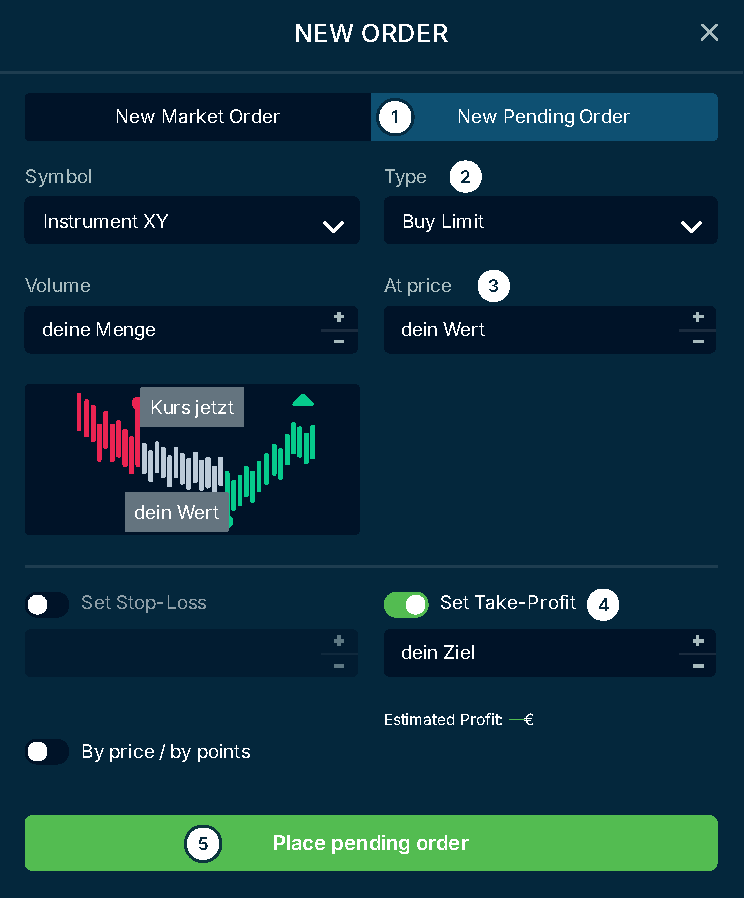
\includegraphics[width=80mm]{fenster-bl.pdf}
\abb{Das Order-Fenster im Reiter New Pending Order}\end{minipage}\hfill
\begin{minipage}[t]{80mm}\vspace{-1mm}\flatter
\begin{enumerate}[label=\protect\cn{\arabic*},leftmargin=7mm,labelsep=3mm,itemsep=3.2mm,topsep=0pt]
\item \ztitel{New Pending Order}\newline{\color{body}\small Wählen Sie den rechten Reiter,
denn nur hier lässt sich ein Aktivierungspunkt hinterlegen, auf den die Plattform wartet. Über
den linken Reiter kaufen oder verkaufen Sie hingegen sofort.}
\item \ztitel{Type}\newline{\color{body}\small Hier wählen Sie einen der vier Ordertypen:
Buy Limit, Sell Limit, Buy Stop oder Sell Stop. Das Bild im Fenster passt sich Ihrer Auswahl an.}
\item \ztitel{At price}\newline{\color{body}\small Tragen Sie hier Ihren Aktivierungspunkt
ein, also den Wert, bei dem die Pending Order ausgelöst wird. Bei Buy Limit liegt er unter dem
aktuellen Kurs.}
\item \ztitel{Set Take-Profit}\newline{\color{body}\small Aktivieren Sie Set Take-Profit und
tragen Sie Ihr Gewinnziel ein. Darunter zeigt die Plattform unter Estimated Profit an, welcher
Gewinn sich daraus ergäbe.}
\item \ztitel{Place pending order}\newline{\color{body}\small Mit diesem Button erteilen Sie
die Order. Von diesem Moment an wartet sie, bis der Markt Ihren Aktivierungspunkt erreicht.}
\end{enumerate}\end{minipage}
\hr
\Htwo{Das Type-Menü und die Regel dahinter}
\noindent\begin{minipage}[t]{46mm}\vspace{0pt}
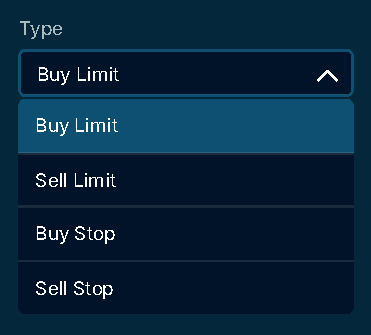
\includegraphics[width=46mm]{type-menu.pdf}
\abb{Ein Klick auf \textbf{Type} öffnet genau diese vier Ordertypen.}
\end{minipage}\hfill
\begin{minipage}[t]{114mm}\vspace{0pt}
% Regel je Ordertyp: Zeilen durch Haarlinien getrennt, Linien oben und unten
{\aktabelle\renewcommand{\arraystretch}{1.75}\setlength{\tabcolsep}{4pt}%
\begin{tabular}{@{}p{26mm}p{42mm}p{40mm}@{}}
\aktoprule
\textcolor{buy}{\bfseries BUY LIMIT} & At price {\bfseries unter} dem Kurs & Take-Profit {\bfseries über} At price \\ \akhaar
\textcolor{sell}{\bfseries SELL LIMIT} & At price {\bfseries über} dem Kurs & Take-Profit {\bfseries unter} At price \\ \akhaar
\textcolor{buy}{\bfseries BUY STOP} & At price {\bfseries über} dem Kurs & Take-Profit {\bfseries über} At price \\ \akhaar
\textcolor{sell}{\bfseries SELL STOP} & At price {\bfseries unter} dem Kurs & Take-Profit {\bfseries unter} At price \\
\akbottomrule
\end{tabular}}
\end{minipage}
\par\akv{1}{\color{body}\small\flatter Entspricht der Wert nicht dieser Regel, bleibt
der grüne Button gesperrt. Beim Wechsel des Ordertyps füllt die Plattform den Wert automatisch
auf der passenden Seite vor. Prüfen Sie ihn dennoch, bevor Sie die Order erteilen.\par}
\clearpage
% -------------------------------------------------------------------------
\kapitel{In der Plattform}
\Hone{Eine wartende Order löschen}
\begin{minipage}{140mm}\lead{Solange eine Pending Order noch nicht ausgelöst wurde, können Sie
sie jederzeit löschen. Die folgenden Schritte beziehen sich auf die mobile Ansicht der
Plattform.}\end{minipage}
\par\akv{2}
\noindent\begin{minipage}{140mm}\flatter
\begin{enumerate}[label=\protect\cn{\arabic*},leftmargin=7mm,labelsep=3mm,itemsep=\LOESCHSEP,topsep=0pt]
\item \ztitel{Orders}\newline{\color{body}Tippen Sie unten in der Navigation auf
Orders; es ist das dritte Symbol.}
\item \ztitel{Pending}\newline{\color{body}Wählen Sie oben den Reiter Pending. Dort
sind die Orders aufgeführt, die noch auf ihren Aktivierungspunkt warten.}
\item \ztitel{Ihre Order}\newline{\color{body}Tippen Sie die Order an, die Sie
löschen möchten. Die Order klappt daraufhin auf und zeigt weitere Angaben, darunter T/P mit
Ihrem Take-Profit. Unterhalb davon erscheinen die Buttons Delete und Modify Order.}
\item \ztitel{Delete}\newline{\color{body}Tippen Sie auf Delete. Die Plattform löscht
die Order nicht sofort, sondern bittet zunächst um eine Bestätigung.}
\item \ztitel{Rückfrage bestätigen}\newline{\color{body}Bestätigen Sie die Rückfrage
mit Delete. Mit Cancel brechen Sie den Vorgang ab, und die Order wartet weiter.}
\end{enumerate}\end{minipage}
\hr
\Htwo{Zum Wortlaut der Rückfrage}
\noindent\begin{minipage}{140mm}\color{body}\flatter In der Rückfrage steht „Are you sure you want to close order at price …?“.
Die Plattform spricht dort von close order; gemeint ist jedoch Ihre wartende Order. Beim
Löschen wird weder gekauft noch verkauft. Anschließend wird die Order auch dann nicht mehr
ausgelöst, wenn der Kurs Ihren Aktivierungspunkt später erreicht.\end{minipage}
\par\akv{1}
\begin{merk}\textbf{Der gesamte Ablauf.} Sie wählen unter \textbf{Type} einen der vier
Ordertypen, tragen bei \textbf{At price} Ihren Aktivierungspunkt ein und legen bei
\textbf{Set Take-Profit} Ihr Gewinnziel fest. Mit \textbf{Place pending order} erteilen Sie die
Order. Anschließend wartet sie, bis der Markt Ihren Aktivierungspunkt erreicht; erst dann wird
gekauft oder verkauft. Möchten Sie nicht länger warten, löschen Sie die Order unter
\textbf{Orders} im Reiter \textbf{Pending}.\end{merk}

\end{document}
